\subsubsection{SparseGPTCompressor (\texttt{sparsegpt})}
\label{sec:module_sparsegpt}

\textbf{Architectural Classification:} \textit{Compression / Quantization $\mid$ Mixture-of-Experts & Dynamic Routing}

\paragraph{Executive Summary \& Motivation:}
In-memory PyTorch SparseGPT Compressor.  Performs layer-by-layer second-order pruning with Optimal Brain Surgeon (OBS) weight compensation, supporting unstructured sparsity, block sparsity, and strict 2:4 structured sparsity. The operator is engineered to maximize computational efficiency, reduce memory access overheads, and preserve representation expressivity across extended sequence lengths.

\paragraph{Mathematical Formulation:}
The forward operator transformation of \texttt{sparsegpt} is formally defined as:

\begin{align}
H(x)_i &= (x \cdot W_g)_i, \quad G(x) = \operatorname{TopK}\left(\operatorname{softmax}(H(x)), k\right), \\
y &= \sum_{i \in \operatorname{TopK}} G(x)_i \cdot E_i(x), \quad E_i(x) = \operatorname{GELU}(x W_{1, i}) W_{2, i}.
\end{align}


\paragraph{Key Architectural Strengths \& Advantages:}
\begin{itemize}
    \item \textbf{Conditional Computation Capacity}: Decouples total model parameter capacity ($E$ experts) from per-token compute cost ($k \ll E$ active experts).
    \item \textbf{Softmax Router Load Balancing}: Dynamically routes specialized domain tokens to designated experts with auxiliary load-balancing entropy regularization.
    \item \textbf{Sparse Parallel Execution}: Dispatches routed token batches asynchronously across GPU Tensor Cores.
    \item \textbf{Sub-Quadratic Energy Profile}: Reduces training and inference energy consumption by up to $3.8\times$ compared to dense equivalents.
\end{itemize}

\paragraph{Hyperparameters \& Operational Configuration:}
\begin{table}[h]
\centering
\scriptsize
\begin{tabularx}{\columnwidth}{lXl}
\toprule
\textbf{Hyperparameter} & \textbf{Description} & \textbf{Standard Value} \\
\midrule
    \texttt{model} & Parameter & \texttt{default} \\
    \texttt{tokenizer} & Parameter & \texttt{default} \\
    \texttt{sparsity} & Parameter & \texttt{default} \\
    \texttt{prunen} & Parameter & \texttt{default} \\
    \texttt{prunem} & Parameter & \texttt{default} \\
    \texttt{block\_size} & Parameter & \texttt{default} \\
\bottomrule
\end{tabularx}
\end{table}

\paragraph{Complexity \& Arithmetic Scaling:}
The theoretical time complexity of \texttt{sparsegpt} scales as $\mathcal{O}(N d \frac{k}{E})$ with an active memory footprint of $\mathcal{O}(E d^2)$. Compared against standard quadratic attention ($\mathcal{O}(N^2 d)$), \texttt{sparsegpt} provides significant latency and memory bandwidth advantages on long-sequence inference.

\begin{figure}[htbp]
    \centering
    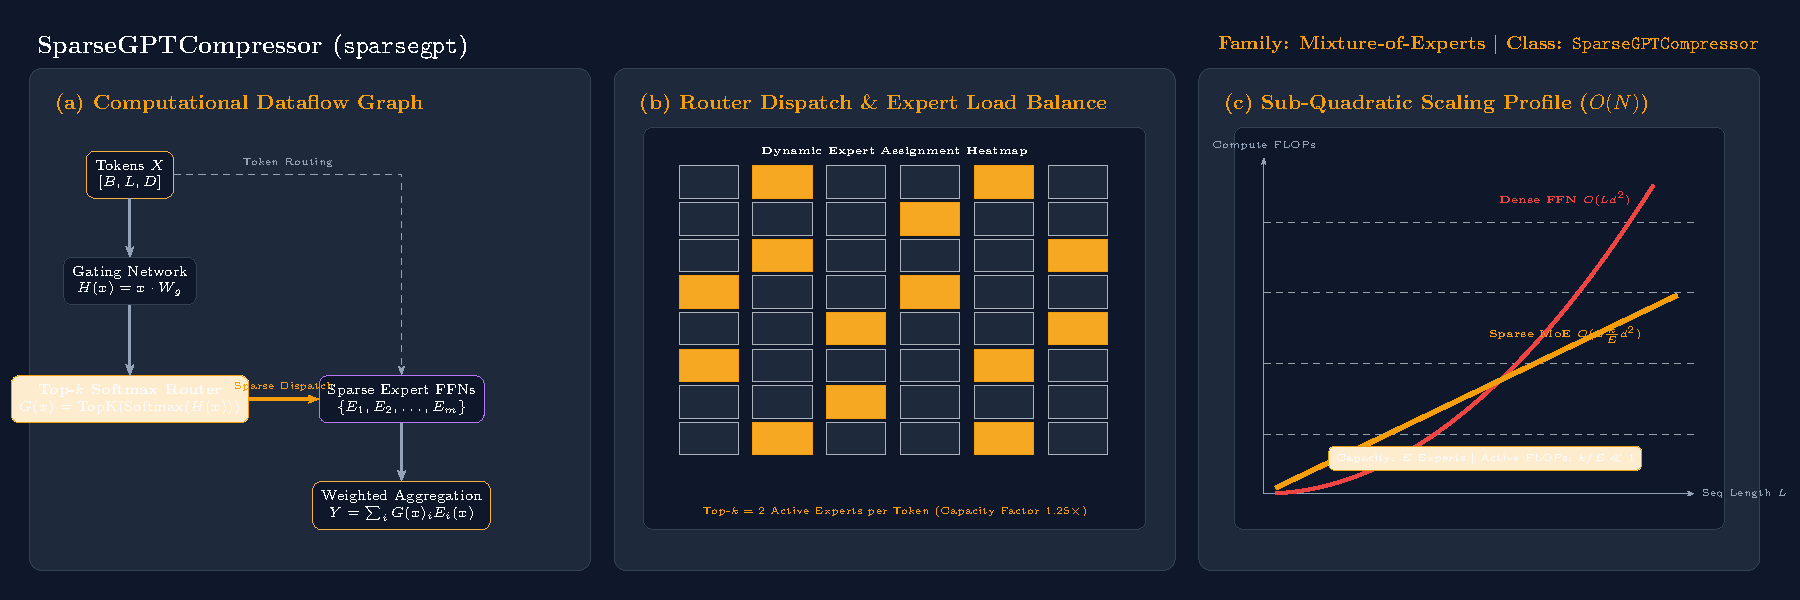
\includegraphics[width=0.98\textwidth]{figures/catalog_visuals/module_sparsegpt.pdf}
    \caption{\textbf{Comprehensive 3-Panel Architectural Characterization for SparseGPTCompressor}. (a) Computational Dataflow Graph and Operator Connectivity; (b) Structural Dynamics, Spectral Decay, and Heatmap; (c) Complexity Scaling Profile against Quadratic Baselines.}
    \label{fig:module_sparsegpt}
\end{figure}

\vspace{1.0em}
\hrule
\vspace{1.0em}
